%\documentclass[11pt]{beamer}
\usepackage[ngerman]{babel}
\usepackage[utf8]{inputenc}
\usepackage{amsmath}
\usepackage{amssymb}
\usepackage{listings} 
\usepackage{stmaryrd}
\lstset{language=Python, tabsize=4, showstringspaces=false,basicstyle=\footnotesize,mathescape=true} 
\lstset{literate=%
  {Ö}{{\"O}}1
  {Ä}{{\"A}}1
  {Ü}{{\"U}}1
  {ß}{{\ss}}1
  {ü}{{\"u}}1
  {ä}{{\"a}}1
  {ö}{{\"o}}1
}
\usepackage{mathtools}
\usepackage{ulem}
\usepackage{tikz}

\usetheme{Boadilla}
\mode<presentation>{
\useoutertheme[subsection=false]{miniframes}
\useinnertheme{rectangles}
%\usecolortheme{crane}
}
\parskip 10pt
\newcommand{\ggT}{\operatorname{ggT}}
\newcommand{\Mod}[3]{#1\equiv#2\text{ mod }#3}
\newcommand{\tmod}{\text{ mod }}


\begin{document}
\title{Vertiefungskurs Mathematik}   
\author{Zahlentheorie - Kongruenz und Restklassen} 
\date{}
\frame{\titlepage} 

%---
\begin{frame}[fragile]

\textbf{Kongruenz}

Definition: Seien $a, b \in \mathbb{Z}, m \in \mathbb{N}$. Dann heißt \textit{a kongruent zu b modulo m} geschrieben: \quad 
\quad $\Mod{a}{b}{m}$, \quad 
 falls $a-b$ durch $m$ teilbar ist. \pause
 
 Beispiel: $m = 5$
 
 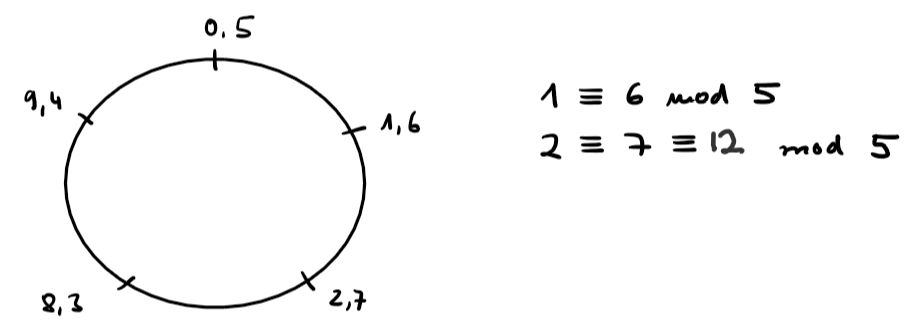
\includegraphics[width=7cm]{bild1.png}
\end{frame}

%---
\begin{frame}[fragile]

Satz: Folgende Aussagen sind äquivalent: \\
(1)  $\Mod{a}{b}{m}$ \\
(2) $\exists k \in \mathbb{Z}: a = b+ km$ \\
(3) Beim Teilen durch $m$ lassen $a$ und $b$ denselben Rest. \pause

Beweis: \\
(1) $\Rightarrow$ (2): $\Mod{a}{b}{m}$ heißt nach Definition $m|(a-b)$. \pause
Also gibt ein $k \in \mathbb{Z}$ mit $k m = a - b.$ \pause Damit gilt: $a = b+ k  m$. \\ \pause
(2) $\Rightarrow$ (3): Sei $r$ der Rest beim Teilen von $a$ durch $m$. \pause Nach dem Satz vom Teilen mit Rest gibt es ein eindeutig bestimmtes $q \in \mathbb{Z}$ mit $a = q  m + r$ und $0 \le r < m$. \pause Damit ist  $b = a - km \pause = q m + r - km\pause =  (q - k)  m + r$. \pause Also lässt auch $b$ beim Teilen durch m den Rest $r$. \\ \pause 
(3) $\Rightarrow$ (1): \pause Es gilt $a = k_1  m + r$ und $b = k_2  m + r$ mit eindeutig bestimmten
$k_1, k_2,r  \in \mathbb{Z}$ und $0 \le r < m$. \pause Also ist $a-b \pause = (k_1-k_2)  m$ \pause und damit gilt $m|(a-b)$. \hfill $\square{}$

\end{frame}

%---
\begin{frame}[fragile]

\textbf{Doppelte Verwendung von `mod'} 

`mod' wird auch als \textit{modulo-Operator} verwendet. 

$r = a \tmod b$ \quad  bedeutet: r ist der Rest bei der Division von a und b. \pause

Beispiel:

$3 = 7 \tmod 2$ \quad bedeutet: 3 ist Rest von 7 : 2 (das ist falsch) \\ \pause
$\Mod{3}{7}{2}$ \quad bedeutet: 3 ist kongruent zu 7 mod 2 (das ist wahr) \pause

Es gilt: $a \tmod m = b \tmod m \Leftrightarrow \Mod{a}{b}{m}$
\end{frame}

%---
\begin{frame}[fragile]

\textbf{Rechenregeln für Kongruenzen} 

Satz: Die Relation `kongruent modulo m' ist eine Äquivalenzrelation auf $\mathbb{Z}$. \\ \pause
(1) $\Mod{a}{a}{m}$ \quad (Reflexivität)  \\ \pause
(2) $\Mod{a}{b}{m}  \Rightarrow \Mod{b}{a}{m}$ \quad (Symmetrie) \\ \pause
(3) $\Mod{a}{b}{m}$ und $\Mod{b}{c}{m}  \Rightarrow \Mod{a}{c}{m}$ \quad (Transitivität) \pause


Satz: Wenn $\Mod{a}{b}{m}$ und $\Mod{c}{d}{m}$, dann gilt: \\
(4) $\Mod{-a}{-b}{m}$ \\  \pause
(5) $\Mod{a+c}{b+d}{m}$ \\ \pause
(6) $\Mod{a\cdot c}{b\cdot d}{m}$ \\ \pause
(7) $\Mod{a^2}{b^2}{m}$,  $\Mod{a^3}{b^3}{m}$, ... \pause

Beweis (nur 6): Aus der Voraussetzung folgt, es gibt $k_1, k_2 \in \mathbb{Z}$ mit $a = b + k_1m$ und $c = d + k_2m$. \pause
Dann ist $ac = ( b + k_1m)( d + k_2m) \pause= bd + bk_2m+k_1md +k_1k_2m^2 = \pause bd +(bk_2 +k_1d +k_1k_2m) 
\cdot m$. \\ \pause
 Das bedeutet: $\Mod{ac}{bd}{m}$ \hfill $\square{}$

\end{frame}

%---
\begin{frame}[fragile]

\textbf{Beispiel} 

$m =7$

$73 + 155 \equiv \pause 3 +1 \equiv 4 \text{ mod }7$ \\ \pause
$73 \cdot 155 \equiv \pause 3 \cdot 1 \equiv 3 \text{ mod }7$ \\ \pause
$73^{155} \equiv \pause 3^ {155} \equiv 5 \text{ mod }7$ 

Nebenrechnung (alles mod 7): \\
$3^1 \equiv 3$ \\
$3^2 \equiv 2$ \\
$3^4 \equiv 4 \equiv 3^{16} \equiv 3^{64}$ \\
$3^8 \equiv 2 \equiv 3^{32} \equiv 3^{128}$ \\
$3^{155} = 3^{128+16+8+2+1} \equiv 2 \cdot 4 \cdot 2 \cdot 2 \cdot 3 \equiv 32 \cdot 3 \equiv -3 \cdot 3 \equiv -9 \equiv 5$
\end{frame}

%---
\begin{frame}[fragile]
\textbf{Teilbarkeitsregeln} 

Satz: Sei $n \in \mathbb{N}$. Dann gilt:

$2|n \Leftrightarrow$ \pause die letzte Ziffer ist gerade. \\
$3|n \Leftrightarrow$ \pause die Quersumme ist durch 3 teilbar. \\
$4|n \Leftrightarrow$  \pause die Zahl aus den letzten beiden Ziffern ist durch 4 teilbar. \\
$5|n \Leftrightarrow$  \pause die letzte Ziffer ist 5 oder 0. \\
$6|n \Leftrightarrow  \pause 2|n$ und $3|n$. \\
$7|n \Leftrightarrow$  \pause die Zahl, die entsteht, wenn man das doppelte der letzten Ziffer von der Zahl ohne die letzte Ziffer abzieht, ist durch 7 teilbar.\\
$8|n \Leftrightarrow$  \pause die Zahl aus den letzten drei Ziffern ist durch 8 teilbar. \\
$9|n \Leftrightarrow$  \pause  die Quersumme ist durch 9 teilbar.\\
$10|n \Leftrightarrow$ \pause  die letzte Ziffer ist eine 0. \\
$11|n \Leftrightarrow$  \pause die alternierende Quersumme ist durch 11 teilbar. \\
$12|n \Leftrightarrow  \pause  3|n$ und $4|n$.  \\

\end{frame}

%---
\begin{frame}[fragile]
\textbf{Beispiele Teilbarkeitsregeln} 

Teilbarkeit durch 7:

$35881 \pause  \rightarrow 3586 \pause  \rightarrow 346 \pause \rightarrow 22 \pause \Rightarrow 7$ kein Teiler von $35881$

Teilbarkeit durch 11:

$355971 \pause : 1-7+9-5+5-3 \pause =  0 \Rightarrow 11|355971$

\end{frame}

%---
\begin{frame}[fragile]
Beweis der Teilbarkeitsregeln (für 3,9,11,7)

Es sei $n = a_ka_{k-1}...a_2a_1a_0$ die Dezimaldarstellung von $n \in \mathbb{N}$ mit $a_i \in \{0,1,...,9\}$ für $0 \le i \le k$.
Dann gilt $n = a_0 + a_1 \cdot 10 + a_2 \cdot 10^2 + ... + a_k \cdot 10^k$  \pause

Teilbarkeit durch 3: $n \equiv a_0 + a_1 \cdot 10 + a_2 \cdot 10^2 + ... + a_k \cdot 10^k$ \\ \pause
$\quad \equiv a_0 + a_1 + a_2  + ... + a_k \pause \equiv$  Quersumme(n) mod 3 \\ \pause
Teilbarkeit durch 9 \pause ebenso. \\ \pause
Teilbarkeit durch 11: $n \equiv a_0 + a_1 \cdot 10 + a_2 \cdot 10^2 + ... + a_k \cdot 10^k$ \\ \pause
$\quad \equiv a_0 - a_1 + a_2  - a_3 + a_4 ... \pause \equiv$  alternierende Quersumme(n) mod 11 \\ \pause
Teilbarkeit durch 7: \pause Es sei $m$ die Zahl $n$ ohne die letzte Ziffer. \pause Dann gilt $n = 10 \cdot m + a_0$. \pause Also gilt auch: 
$2n = 20m + 2a_0$. \pause Und damit gilt: $2n = 21m - m + 2a_0$. \pause
Daraus folgt: $2n \equiv -m +2a_0 \text{ mod }7$. \pause Insgesamt gilt: 
$7|n \Leftrightarrow 7|2n \pause \Leftrightarrow   \Mod{-m +2a_0 }{0}{7} \pause \Leftrightarrow   \Mod{m -2a_0 }{0}{7} \pause \Leftrightarrow 7|(m-2a_0) \pause \square{}$

\end{frame}

%---
\begin{frame}[fragile]
\textbf{Restklassen} 

Betrachte alle Zahlen, die beim Teilen durch eine Zahl $m \in \mathbb{N}$ denselben Rest lassen. Diese Zahlen werden zu einer
Menge zusammengefasst, der Restklasse. \pause

Definition: Die \textit{Restklasse} $\overline{a}$ von $a$ modulo $m$ ist definiert durch: \\
$\overline{a} = \{b \in \mathbb{Z}: \Mod{b}{a}{m}\}$. \pause

Andere Schreibweise: $[a]$ statt $\overline{a}$. \pause

Beispiel: Die Restklassen modulo 5 sind

$\overline{0} = \{ ..., -10, -5, 0, 5, 10, ....\}$ \\
$\overline{1} = \pause \{ ..., -9, -4, 1, 6, 11, ....\}$ \\
$\overline{2} = \pause  \{ ..., -8, -3, 2, 7, 12, ....\}$ \\
$\overline{3} = \{ ..., -7, -2, 3, 8, 13 ....\}$ \\
$\overline{4} = \{ ..., -6, -1, 4, 9, 14 ....\}$ \\

\end{frame}
 
 %---
\begin{frame}[fragile]

\textbf{Rechnen im Restklassenring}

Die Menge aller Restklassen modulo m heißt \textit{Restklassenring modulo m} geschrieben  $\mathbb{Z}_m$. \pause

Beispiel:  $\mathbb{Z}_5 =\{ \overline{0}, \overline{1}, \overline{2},\overline{3}, \overline{4} \} $ \pause

Definition: Seien $a,b \in \mathbb{Z}$. \\
$\overline{a} + \overline{b} := \overline{a+b}$ \\
$\overline{a} \cdot \overline{b} := \overline{a \cdot b}$  \pause

Beispiel in  $\mathbb{Z}_5$: $\overline{2} + \overline{3} = \overline{5}$ 
\quad $\overline{7} + \overline{8} = \overline{15} = \overline{5}$\\ \pause
Es spielt keine Rolle, welcher Repräsentant der Restklasse für die Berechnung genommen wird. Addition und Multiplikation sind  `wohldefiniert'.

\end{frame}


 %---
\begin{frame}[fragile]

\textbf{Verknüpfungstabellen}

Die Verknüpfungstabelle für Addition und Multiplikation in $\mathbb{Z}_5$

\begin{tabular}{ll}
\begin{tabular}{l|lllll}
$+$ & $0$ & $1$ & $2$ & $3$ & $4$ \\ \hline
0 & $0$ & $1$ & $2$ & $3$ & $4$ \\
1 & $1$ & $2$ & $3$ & $4$ & $0$ \\
2 & $2$ & $3$ & $4$ & $0$ & $1$ \\
3 & $3$ & $4$ & $0$ & $1$ & $2$ \\
4 & $4$ & $0$ & $1$ & $2$ & $3$ \\
\end{tabular}
&\quad
\begin{tabular}{llllll}
* & $0$ & $1$ & $2$ & $3$ & $4$ \\ \hline
$0$ & $0$ & $0$ & $0$ & $0$ & $0$ \\
$1$ & $0$ & $1$ & $2$ & $3$ & $4$ \\
$2$ & $0$ & $2$ & $4$ & $1$ & $3$ \\
$3$ & $0$ & $3$ & $1$ & $4$ & $2$ \\
$4$ & $0$ & $4$ & $3$ & $2$ & $1$ \\
\end{tabular}
\end{tabular}

\end{frame}

%---
\begin{frame}[fragile]
Subtraktion: $\overline{a} - \overline{b} := \overline{a}+ \overline{-b}$. Dann gilt: $\overline{a} - \overline{a} = \overline{a}+ \overline{-a}=$ 
$\overline{a-a} = \overline{0}$ \pause

Hilfsfrage für negative Restklassen: Wieviel fehlt vom Absolutbetrag zum nächsten Vielfachen von m? \quad
Beispiel in  $\mathbb{Z}_7$: $\overline{-25}= \pause \overline{3}$ \pause

Division in $\mathbb{Z}_5:$ \\~\\
$ \dfrac{\overline{1}}{\overline{2}} = x \pause \Leftrightarrow \overline{1} = \overline{2} \cdot x  \Leftrightarrow \pause x= \overline{3}$ \pause
\\~\\
$ \dfrac{\overline{2}}{\overline{3}} \pause = x \Leftrightarrow \overline{2} = \overline{3} \cdot x  \Leftrightarrow x= \overline{4}$ 

\end{frame}

%---
\begin{frame}[fragile]
Problem bei der Division in $\mathbb{Z}_4:$ 

\begin{tabular}{lllll}
* & $0$ & $1$ & $2$ & $3$ \\ \hline
$0$ & $0$ & $0$ & $0$ & $0$ \\
$1$ & $0$ & $1$ & $2$ & $3$ \\
$2$ & $0$ & $2$ & $0$ & $2$ \\
$3$ & $0$ & $3$ & $2$ & $1$ \\
\end{tabular}

$ \dfrac{\overline{1}}{\overline{2}} = x \Leftrightarrow \overline{1} = \overline{2} \cdot x$\pause, \quad es gibt kein x. 
\\~\\
$ \dfrac{\overline{2}}{\overline{2}} = x \Leftrightarrow \overline{2} = \overline{2} \cdot x$\pause, \quad $x=\overline{1}$ oder $x=\overline{3}$, d.h. x ist nicht eindeutig.

\end{frame}

%---
\begin{frame}[fragile]
\textbf{Existenz von Brüchen in $\mathbb{Z}_m$ } \pause

$ \dfrac{\overline{a}}{\overline{b}} = \overline{x} \pause \Leftrightarrow \overline{a} = \overline{b} \cdot \overline{x} \pause = \overline{b \cdot x} \pause
 \Leftrightarrow \Mod{a}{bx}{m}  \pause \Leftrightarrow \exists k \in \mathbb{Z}: km = a-bx$  \pause
 
 In der letzten Gleichung sind $a, b, m$ vorgegeben $k$ ist unbekannt und $x$ ist gesucht. \pause Wir müssen also die diophantische Gleichung  $bx+km=a$ lösen. \pause
 
 Falls $m$ Primzahl, dann ist $\ggT(m,b) = 1$. \pause Dann hat die Gleichung für jedes $a$ eine Lösung $x_0$ \pause und alle anderen Lösungen sind gegeben
 durch $x_0 + t\cdot m, t \in \mathbb{Z}$. \pause Dies sind die Elemente von $\overline{x_0}$.

\end{frame}

%---
\begin{frame}[fragile]
\textbf{Satz vom Dividieren}: Sei $p$ Primzahl, $a \in \mathbb{Z}, b \in \{1,...,p-1\}$, dann besitzt die Gleichung 
$\overline{b} \cdot \overline{x} = \overline{a}$ in  $\mathbb{Z}_p$ genau eine Lösung $\overline{x}$, \pause  d.h.   $\dfrac{\overline{a}}{\overline{b}}: = \overline{x}$ ist definiert. \pause

Merkregel: Wenn wir $ \dfrac{\overline{1}}{\overline{a}}$ in $\mathbb{Z}_p$ suchen, dann lösen wir die Gleichung $ax + py = 1$. Es gilt dann:
$\dfrac{\overline{1}}{\overline{a}} = \overline{x}$. \pause

Beispiel: Bestimme $ \dfrac{\overline{1}}{\overline{7}}$ in $\mathbb{Z}_{11}$. \pause Wir lösen die Gleichung $7x + 11y = 1$.
\pause Eine Lösung ist $x=-3, y=2$. \pause Also gilt: $\dfrac{\overline{1}}{\overline{7}} = \overline{-3} = \overline{8}$.
\end{frame}

%---
\begin{frame}[fragile]
\textbf{Kleiner Satz von Fermat:} \\
Sei $p$ Primzahl, $a \in \mathbb{N}$ kein Vielfaches von $p$. \\
Dann gilt: $\overline{a}^{p-1} = \overline{1}$ in $\mathbb{Z}_p$ \quad bzw. $\Mod{a^{p-1}}{1}{p}.$  \pause

Beispiel in  $\mathbb{Z}_5$: 
$2^4 \equiv \pause 16 \equiv 1$, \quad $3^4 \equiv \pause  81 \equiv 1$, \quad $4^4  \equiv \pause (-1)^4 \equiv 1$ \pause

Beweis: Setze $A = \{\overline{0a}, \overline{1a}, \overline{2a},...,\overline{(p-1)a}\} \subseteq \mathbb{Z}_p$. \pause
Wir zeigen zunächst $A = \mathbb{Z}_p$, indem wir zeigen, dass alle Elemente in $A$ verschieden sind. \\ \pause
Annahme: $\overline{ja} = \overline{ka}$ für ein $k >j$. \pause Dann gilt: $\overline{0}=\overline{ja}-\overline{ka} \pause = \overline{ja-ka} = \pause \overline{(j-k)a}$. \pause Da $j-k \neq 0$ können wir dividieren und erhalten $\overline{a}= \frac{\overline{0}}{\overline{j-k}}$. \pause Damit ist $a$ ein Vielfaches von p, im Widerspruch zur Annahme. \pause Also gilt $A = \mathbb{Z}_p$.
\pause Wir entfernen $\overline{0a}$ aus $A$ und $\mathbb{Z}_p$. \pause Das Produkt der restlichen Elemente muss gleich sein. \pause $\overline{1a} \cdot \overline{2a} \cdot ... \cdot \overline{(p-1)a} = \overline{1} \cdot \overline{2} \cdot ... \cdot \overline{p-1}$. \pause
Wir dividieren durch $\overline{1}, \overline{2}, ...$ und erhalten: \quad $\overline{a}^{p-1} = \overline{1}$ \pause \hfill $\square{}$
\end{frame} 

%---
\begin{frame}[fragile]
\textbf{Primitivwurzeln}: 

Definition: Ein Element $\overline{g} \in  \mathbb{Z}_m$ heißt \textit{Primitivwurzel}, falls durch $\overline{g}^k$ alle Elemente von $\mathbb{Z}_m$ außer
$\overline{0}$ dargestellt werden können. \pause

Beispiel:

\begin{tabular}{ll}
$2^0 \equiv 1 \text{ mod } 7$ &\quad $3^0 \equiv 1 \text{ mod } 7$ \\
$2^1 \equiv 2  $ &\quad $3^1 \equiv 3$ \\
$2^2 \equiv 4  $ &\quad $3^2 \equiv 2$ \\
$2^3 \equiv 1  $ &\quad $3^3 \equiv 6$ \\
$2^4 \equiv 2  $ &\quad $3^4 \equiv 4$ \\
$2^5 \equiv 4  $ &\quad $3^5 \equiv 5$ \\
$2^6 \equiv 1  $ &\quad $3^6 \equiv 1$ 
\end{tabular} \pause

$\overline{3}$ ist Primitivwurzel in $ \mathbb{Z}_7$,  $\overline{2}$ nicht. \pause

Tritt bei $\overline{g}^k$ vor $\overline{g}^{p-1}$ die Restklasse $\overline{1}$ auf, so wiederholen sich die Restklassen. Es kann keine Primitivwurzel vorliegen.
\end{frame}
 
\end{document}